\documentclass[tikz,border=6pt]{standalone}
\usepackage{amsmath}
\usetikzlibrary{calc}

% ---------- Styles & helpers ----------
\newcommand{\bit}[4][violet]{%
  % #1 color (default violet), #2 x, #3 y, #4 label
  \node[
    draw=#1!70!black,
    rounded corners=2pt,
    very thick,
    top color=#1!10,
    bottom color=#1!45,
    shading=axis,
    minimum width=6.2mm,
    minimum height=6.2mm,
    inner sep=0pt,
    font=\footnotesize\sffamily\bfseries,
    text=#1!60!black,
    align=center
  ] at (#2,#3) {#4};
}

\begin{document}
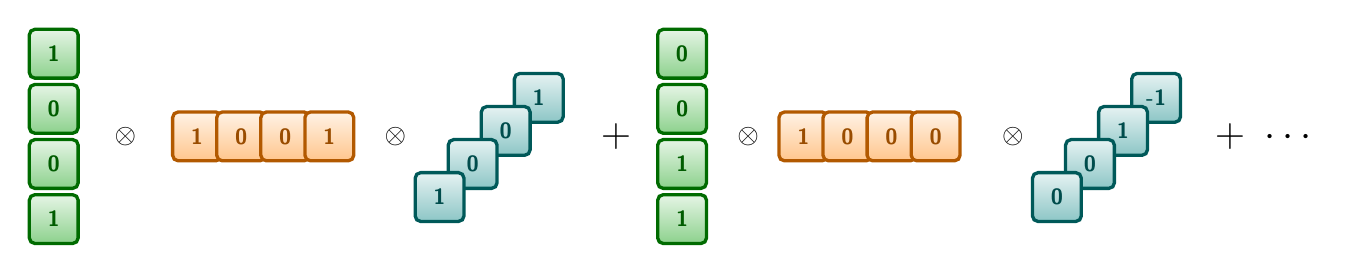
\begin{tikzpicture}[x=7mm,y=7mm]

% nicer symbol nodes
\tikzset{
  circop/.style={draw=black!50, circle, minimum size=9.5mm, thick, font=\Large},
  plus/.style={font=\Large},
}

% ---------------- Term 1: ----------------
% left vertical (purple): 1,0,0,1
\bit[green!60!black]{0}{3}{1};
\bit[green!60!black]{0}{2}{0};
\bit[green!60!black]{0}{1}{0};
\bit[green!60!black]{0}{0}{1};

\node at (1.3,1.5) {$\otimes$};

% middle horizontal (green): 1,0,0,1
\bit[orange]{2.6}{1.5}{1};
\bit[orange]{3.4}{1.5}{0};
\bit[orange]{4.2}{1.5}{0};
\bit[orange]{5.0}{1.5}{1};

\node at (6.2,1.5) {$\otimes$};

% right slanted (blue-purple): 1,0,1
\bit[teal]{8.8}{2.2}{1};
\bit[teal]{8.2}{1.6}{0};
\bit[teal]{7.6}{1.0}{0};
\bit[teal]{7.0}{0.4}{1};

\node[plus] at (10.2,1.5) {$+$};

% ---------------- Term 2: ----------------
% left vertical (purple): 1,0,0,1
\bit[green!60!black]{11.4}{3}{0};
\bit[green!60!black]{11.4}{2}{0};
\bit[green!60!black]{11.4}{1}{1};
\bit[green!60!black]{11.4}{0}{1};

\node at (12.6,1.5) {$\otimes$};

% middle horizontal (green): 1,0,0,0
\bit[orange]{13.6}{1.5}{1};
\bit[orange]{14.4}{1.5}{0};
\bit[orange]{15.2}{1.5}{0};
\bit[orange]{16.0}{1.5}{0};

\node at (17.4,1.5) {$\otimes$};

% right slanted (blue-purple): 0,1,1
\bit[teal]{20.0}{2.2}{-1};
\bit[teal]{19.4}{1.6}{1};
\bit[teal]{18.8}{1.0}{0};
\bit[teal]{18.2}{0.4}{0};

\node[plus] at (22.0,1.5) {$+\ \cdots$};

\end{tikzpicture}
\end{document}
